\def\mytitle{Circle Assignment}
\def\myauthor{A.Gowri Priya}
\def\contact{gowripriyaappayyagari@gmail.com}
\def\mymodule{Future Wireless Communication (FWC)}
\documentclass[10pt, a4paper]{article}
\usepackage[a4paper,outer=1.5cm,inner=1.5cm,top=1.75cm,bottom=1.5cm]{geometry}
\twocolumn
\usepackage{setspace}
\usepackage{graphicx}
\graphicspath{{./images/}}
\usepackage[colorlinks,linkcolor={black},citecolor={blue!80!black},urlcolor={blue!80!black}]{hyperref}
\usepackage[parfill]{parskip}
\usepackage{lmodern}
\usepackage{tikz}
	\usepackage{physics}
%\documentclass[tikz, border=2mm]{standalone}
\usepackage{karnaugh-map}
\usepackage{tabularx}
\usetikzlibrary{calc}
\usepackage{amsmath}
\usepackage{amssymb}
\renewcommand*\familydefault{\sfdefault}
\usepackage{watermark}
\usepackage{lipsum}
\usepackage{xcolor}
\usepackage{listings}
\usepackage{float}
\usepackage{titlesec}
\providecommand{\mtx}[1]{\mathbf{#1}}
\titlespacing{\subsection}{1pt}{\parskip}{3pt}
\titlespacing{\subsubsection}{0pt}{\parskip}{-\parskip}
\titlespacing{\paragraph}{0pt}{\parskip}{\parskip}

\newcommand{\myvec}[1]{\ensuremath{\begin{pmatrix}#1\end{pmatrix}}}
\let\vec\mathbf
\lstset{
frame=single, 
breaklines=true,
columns=fullflexible
}

\title{\mytitle}
\author{\myauthor\hspace{1em}\\\contact\\FWC22012\hspace{6.5em}IITH\hspace{0.5em}\mymodule\hspace{6em}ASSIGN-5}
\date{}
\begin{document}
	\maketitle
\section{Problem}
The length of the diameter of the circle which touches the x-axis at the point (1,0) and passes through the point (2,3) is?
\section{Construction}
\begin{figure}[h]
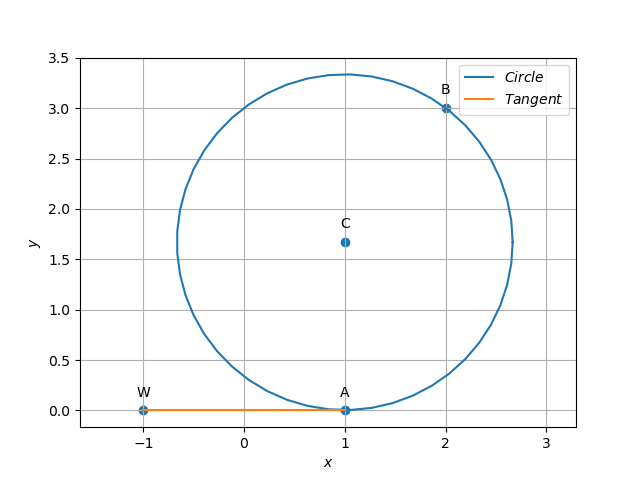
\includegraphics[scale=0.5]{cir.png} 
\end{figure}
\section{Solution}
The equation of the circle is 
\begin{equation}
	x^T\vec{V}x + 2\vec{u}^Tx + f = 0
\end{equation}
Circle passes through $\myvec{2\\3}$ and  touches the x-axis at $\myvec{1\\0}$ 
Let $\vec{A}$=$\myvec{1\\0}$ and $\vec{B}$=$\myvec{2\\3}$ and  $\vec{m}$=$\myvec{1\\0}$
\begin{equation}
	\vec{A}\vec{A}^T + 2\vec{u}^T\vec{A} + f = 0
\end{equation}
\begin{equation}
	\norm{\vec{A}}^2 + 2\vec{A}^T \vec{u} + f = 0
\end{equation}
\begin{equation}
	\myvec{2\vec{A}^T & 1}\myvec{\vec{u} \\ f} = -\norm{A}^2 
\end{equation}
\begin{equation}
	\vec{B}\vec{B}^T + 2\vec{u}^T\vec{B} + f = 0
\end{equation}
\begin{equation}
	\norm{\vec{B}}^2 + 2\vec{B}^T\vec{u} + f = 0
\end{equation}
\begin{equation}
	\myvec{2\vec{B}^T & 1}\myvec{\vec{u} \\ f} = -\norm{\vec{B}}^2
\end{equation}
The equation of the tangent is
\begin{equation}
	\vec{m}^T (\vec{V}q + \vec{u}) = 0
\end{equation}
\begin{equation}
	\vec{m}^T\vec{A} +\vec{m}^T\vec{u} = 0
\end{equation}
\begin{equation}
	 \vec{m}^T\vec{u} = -\vec{m}^T\vec{A}
\end{equation}
from equations (4),(7) and (10),we can write as 
\begin{equation}
	\myvec{\vec{m}^T & 0 \\ 2\vec{A}^T & 1 \\ 2\vec{B}^T & 1}\myvec{\vec{u} \\ f} = \myvec{-\vec{m}^T\vec{A} \\ -\norm{\vec{A}}^2 \\ -\norm{\vec{B}}^2}
\end{equation}
\begin{center}
$\myvec{1&0&0&-1 \\2 & 0& 1 & -1 \\ 4 & 6 & 1 & -13 } \xrightarrow[]{R_2 \leftarrow R3 }$\\
$\myvec{1&0&0&-1 \\4 & 6 & 1 & -13 \\ 2 & 0 & 1 & -1 } \xrightarrow[]{R_2 \leftarrow R2 / 6 } $\\
$\myvec{1&0&0&-1 \\4/6 & 1 & 1/6 & -13/6 \\ 2 & 0 & 1 & -1 } \xrightarrow[]{R_3 \leftarrow  R_3-2R_1 }$\\
$\myvec{1&0&0&-1 \\4/6 & 1 & 1/6 & -13/6 \\ 0 & 0 & 1 & 1 } \xrightarrow[]{R_2 \leftarrow R_2- 4/6R_1 }$\\
$\myvec{1&0&0&-1 \\0 & 1 & 1/6 & -9/6 \\ 0 & 0 & 1 & 1 } \xrightarrow[]{R_2 \leftarrow R_2- 1/6R_3 }$\\
$\myvec{1&0&0&-1 \\0 & 1 & 0 & -10/6 \\ 0 & 0 & 1 & 1 }$\\
\end{center}
By solving the above equations\\\\ $\vec{u} =\myvec{-1 \\ -10/6}=\myvec{-1 \\ -5/3}$\\\\\\
The center is $\vec{C}$=-$\vec{u}$\\\\
$\therefore$ $\vec{C} = \myvec{1\\ 5/3}$
 and $f = 1$ \\
\begin{equation}
	Radius\;(R) =\sqrt{\vec{u^T}.\vec{u}-f}
\end{equation}
\begin{equation}                                                                                   \sqrt{\myvec{-1 &-5/3}\myvec{-1\\-5/3}-1} =5/3                                        
\end{equation}
$\therefore$ R=5/3=1.67\\\\
D=2*R\\\\
$\therefore$ Diameter (D)=3.34
\section{Execution}
Verify the above problem in the following code.\\
\framebox{
\url{https://github.com/gowripriya-2002/FWC/blob/main/Matrix/circle_assignment/codes/circle.py}}	
\bibliographystyle{ieeetr}
\end{document}
